% PLEASE USE THIS FILE AS A TEMPLATE
% Check file iosart2c.tex for more examples
%
% Journal:
%   Journal of Ambient Intelligence and Smart Environments (jaise)
%   Web Intelligence and Agent Systems: An International Journal (wias)
%   Semantic Web: Interoperability, Usability, Applicability (SW)
% IOS Press
% Latex 2e

% options: jaise|wias|sw
% add. options: [seceqn,secfloat,secthm,crcready,onecolumn]


%\documentclass{iosart2c}

\documentclass[sw]{iosart2c}
%\documentclass[wias]{iosart2c}
%\documentclass[jaise]{iosart2c}

\usepackage[T1]{fontenc}
\usepackage{times}%
\usepackage{natbib}% for bibliography sorting/compressing
%\usepackage{amsmath}
%\usepackage{endnotes}
\usepackage{graphics}

\usepackage{color}
\usepackage{url}

%%%%%%%%%%% Put your definitions here

\newcommand{\myurl}[1]{\footnote{\url{#1}}}
\newcommand{\todo}[1]{\textbf{{\color{blue}$\Longrightarrow$ #1}}}


%%%%%%%%%%% End of definitions

\pubyear{0000}
\volume{0}
\firstpage{1}
\lastpage{1}

\begin{document}

\begin{frontmatter}

%\pretitle{}
\title{Plant-Pathogen Interactions Ontology (PPIO)}
\runningtitle{}
%\subtitle{}

%\review{}{}{}


% For one author:
%\author{\fnms{} \snm{}\thanks{}}
%\address{}
%\runningauthor{}

%Two or more authors:
\author[A]{\fnms{Alejandro} \snm{Rodr\'iguez Iglesias}\thanks{Corresponding author. Email:alejandroriglesias@gmail.com}},
\author[A]{\fnms{Mikel} \snm{Ega\~na Aranguren}}
\author[A]{\fnms{Alejandro} \snm{Rodr\'iguez Gonz\'alez}}
\author[A]{\fnms{Mark D.} \snm{Wilkinson}}
\runningauthor{}
\address[A]{Biological Informatics Group, Centre for Plant Biotechnology and Genomics (CBGP), Technical University of Madrid (UPM), Spain}
%\address[B]{}

\begin{abstract}
Plant-pathogen interactions are an important knowledge domain within plant biology and biotechnology, both scientifically and in economic terms. Unlike other knowledge domains within   life sciences, however, semantic technologies have not been used extensively to codify it; therefore, there is a lack of axiomatic models amenable to automated integration and inference. We present the Plant-Pathogen Interactions Ontology (PPIO), a first step towards the axiomatization of plant-pathogen interactions knowledge. PPIO encourages consistent annotation and supports both query and inference.
\end{abstract}

\begin{keyword}
 Plant pahogenic bacteria \sep Ontologies \sep Semantic Web \sep PPIO
\end{keyword}

\end{frontmatter}

%%%%%%%%%%% The article body starts:

\section{Introduction}\label{s1}

Many bacterial genera are responsible for causing diseases in a wide range of plant species \cite{Mansfield}, and if the different levels of the host defense barriers are overcomed by the pathogen, the infection process can ultimately lead to the death of the plant. This phenomenon can affect crop yield, which automatically will translate into considerable economic loss. On the other hand, in the context of challenges such as feeding a growing world population, and the trend of emerging economies to consume more meat, where animal feed increases the consumption per capita of available food-crops, it is crucial that we identify ways to increase the productivity of crop fields \cite{Montesinos}. Therefore, being able to accurately record, explore, and query biological data regarding plant-pathogen interactions is a necessary step towards the improvement and protection of these important plant species. This issue continues being subject of intensive research worldwide. This is documented in hundreds of articles that focus on the biological consequences and the mechanisms of pathogenic bacteria interactions with their hosts \cite{DeWit} \cite {Dodds}. 


Certain semantics-oriented projects are particularly noteworthy as a result of their success in using semantics to aid in automated data  integration from non-collaborating resources, like the OBO foundry \cite{Smith},which includes Gene Ontology (GO) \cite{Gene}, Bio2RDF \cite{RDF} and the W3C Semantic  Web  for Health  Care  and  Life Sciences Interest Group\myurl{http://www.w3.org/blog/hcls/}. In the context of plant biotechnology and phytopathology, however, semantic technologies have been applied to only a limited number of domain resources. For example, the Plant Ontology Consortium developed the Plant Ontology\myurl{tp://www.plantontology.org/} platform to describe the anatomy, morphology and developmental stages of plants \cite{PO}. The Plant Trait Ontology \cite{PTO}, related to the Gramene project\myurl{http://www.gramene.org}, defines a vocabulary for describing the specific appearance or qualities of various plant anatomical structures. The Plant Disease Ontology (IDOPlant) \cite{Walls}, was modeled after the human Infectious Diseases Ontology (IDO) \cite{IDO} to serve as a reference ontology that contained and covered any plant infectious disease. Apart from IDOPlant, there is another contribution directly related to the plant-pathogenic bacteria area, and is the GO extension for description of the Type III Effectors \cite{Lindeberg}, which is part of the Plant-Associated Microbe Gene Ontology project (PAMGO). 


As just discussed, Semantic technologies have proven extremely effective and have widely adopted in other branches of the life sciences community. However, they have not been extensively applied to the knowledge domain of plant-pathogenic bacteria to date. Despite the clear need for automation of data annotation, categorization, integration, interpretation, and quality-control, the data and knowledge in this domain remains largely computationally opaque, limiting the utility and usability of these important datasets. Here we present the Plant Pathogen Interactions Ontology (PPIO), an ontological platform that integrates data related to plant pathology and physiology in the context of pathogenic interactions. The aim of PPIO is to leverage this combined knowledge to assist in the interpretation of the phenotypic responses that result from plant-pathogenic bacteria interactions. This platform offers an axiomatic scaffold into which biologically relevant data can be embedded in a precise and computationally-effective accessible manner. 

%\subsection{}\label{s1.1}



\section{Modelling}

The initial data necessary to start building the ontology was collected manually by consulting a number of different of web resources. The web page http://pseudomonas-syringae.org/ was the starting point; it contains diverse pieces of state-of-art information related with various {\itshape Pseudomonas syringae} strains. This web page was a bridge to other web resources where more datasets were collected, like the (NCPPB, etc). After an initial collection of data was gathered, the modelling of these datasets was performed using the ontology editor Prot\'eg\'e (version). 

\subsection{Desing principles}

The main goal pursued during the modelling and designing process was to semantically capture as many biological data existing as possible, and special effort is being done in accurately modelling the {\itshape disease triangle} \myurl{http://www.apsnet.org/edcenter/instcomm/TeachingArticles/Pages/DiseaseTriangle.aspx} . This term is one of the most essential milestones in the plant pathology ambit, and it principal statement asserts that three factors must be present for a disease to occur: the virulent pathogen, a susceptible host and a propitious environment for disease progression. Two classes have been created to represent these three elements, the {\sf Environmental\_parameter} and the {\sf Organism} classes. (introducing more text here about the relation of these classes).
Physiological state of plants can be inferred visually by observing plant phenotypes. Thus, significant work/endeavour is also being done in the modelling of plant phenotypic representations in PPIO. To this end, a number of classes have been specifically created to represent plant phenotypic traits in a precise and pertinent manner, being especially important the Phenotpyic process and the Phenotype? Classes (figura con un esquema de la jerarquía de clases). These two classes semantically illustrate the output of the interaction between the host and the bacteria. 


\section{Creation methodology}


\subsection{Ontology production}

The development of PPIO is automated as much as possible. Once the main structure is set manually, the remaining parts are produced programmatically by introducing the ontology in a tailored Galaxy \cite{galaxy} workflow that adds the necessary entities and axioms (Figure \ref{fig:galaxy-workflow}). By using Galaxy, the specific workflow we need is defined once and it can be executed for each release: complex modifications of the ontology can be defined in the Ontology Pre Procesoor Language (OPPL)\myurl{http://oppl.sf.net} and executed in every release easily. The galaxy workflow can be reproduced at \url{http://biordf:8090 ...} \todo{AleJr add PUBLIC url of the workflow} with any ontology and/or OPPL script. The galaxy workflow comprises two main steps:

\begin{enumerate}

\item The organism taxa hierarchy is produced by the Galaxy tool NCBITaxonomy2OWL\myurl{https://github.com/wilkinsonlab/NCBITaxonomy2OWL}: NCBITaxonomy2OWL gets the user-defined taxa from a BioPortal Web Service \cite{bioportal} and injects them in the target ontology, reproducing the original taxonomical hierarchy (represented as a simple class-subclass hierarchy \cite{taxa_ismb_2008}) and adding each taxon with a resolvable OntoBee\myurl{http://www.ontobee.org/} URI.

\item OWL Puning\myurl{http://www.w3.org/TR/owl2-new-features/Punning} is used in the X hierarchy of PPIO to represent X classes both as OWL classes and individuals, in order to link pathogens, which are individuals, with symptons and taxononmies??. This is achieved by defining two OPPL scripts and executing them via OPPL-Galaxy \cite{OPPL-Galaxy-JBMS}:

{\small 
\begin{verbatim}
?x:CLASS,
?y:INDIVIDUAL = create(?x.RENDERING)
SELECT ?x SubClassOf NCBITaxon_1
WHERE ?x != Nothing, ?x != Thing
BEGIN
ADD ?y Type ?x
END;
\end{verbatim}
}

{\small 
\begin{verbatim}
?x:CLASS,
?y:INDIVIDUAL = create(?x.RENDERING)
SELECT ?x SubClassOf PPIO_0000069
WHERE ?x != Nothing, ?x != Thing
BEGIN
ADD ?y Type ?x
END;
\end{verbatim}
}

\end{enumerate}

\begin{figure}
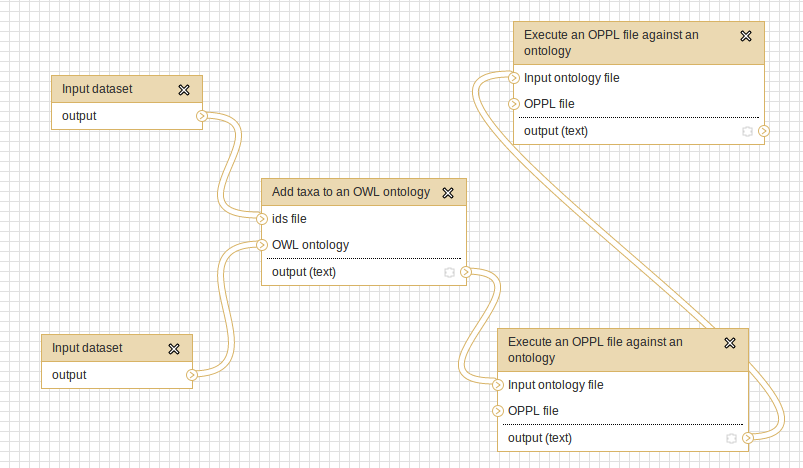
\includegraphics{galaxy-workflow}
\caption{Galaxy workflow that produces the final version of PPIO \todo{AleJr, change by real image}.}\label{fig:galaxy-workflow}
\end{figure}

\subsection{URIs}
PPIO follows the best practice of assigning a numerical ID to each entity, obatining a URI of the type \url{http://purl.oclc.org/PPIO#PPIO_NNNNNNN} (REF). Every entity (classes, individuals and object properties) has an informative rdfs:label. The ontology URI (\url{http://purl.oclc.org/PPIO}) is HTTP resolvable and permanent (the PURL server redirects to our current server at \url{biordf.org}). 




\section{Discussion}

Although the existence of ontologies related with plants and plant pathology has already been reported \cite{PTO} \cite{Lindeberg} \cite{Walls}, the justification for building this ontology lies in its coverage of a domain not fully represented by other resources. In a comparison between the IDOPlant and PPIO, a more generalistic approach of data modelling can be seen in the case of the first platform, which semantically describes plant infectious diseases caused by either biotic or abiotic agents . The ontology reported here pursues a knowledge capture strategy specifically focused on data that concerns plant-pathogenic bacteria interactions. On the other hand, although the GO extension for the type III effectors is built for capturing processes in the host-pathogen level, effector proteins data capture is emphasized. Of course, PPIO has been developed in order to be used with these ontological resources. In this aspect, PPIO complements these previous ontologies by introducing accurate and concrete biological information concerning plant pathogenic bacteria and the interactions with plants. The final goal of this initiative is to use this platform, combined with others, as a diagnosis/prevention/alert system. PPIO will make it possible for users to pose, and answer, questions like the following ones and obtain a meaningful answer:

\begin{enumerate}
\item Is tomato plant susceptible to the attack of {\itshape Pseudomonas syringae} pv. {\itshape tomato} DC3000?
\item Does a high humidity and and low temperature rates favour the development of {\itshape Pectobacterium carotovorum} subsp. {\itshape carotovorum}?
\item What is the phenotype of the disease produced by {\itshape Dickeya dadantii} in {\itshape Solanum tuberosum}?

\end{enumerate}

A new knowledge capture project is now being developed in the laboratory, and it is our thought that it will aid in the process of collecting as many data as possible. This project starts from the idea that the participation of field experts should ensure the fiability of the PPIO data content.

\section*{Acknowledgements}
Alejandro Rodr\'iguez Iglesias and Alejandro Rodr\'iguez Gonz\'alez are funded by the Isaac Peral Programme. Mark D. Wilkinson and Mikel Ega\~na Aranguren are funded by the Marie Curie-COFUND Programme (FP7) of the EU.



%\begin{figure}[t]
%\includegraphics{}
%\caption{Figure caption.}\label{f1}
%\end{figure}

%\begin{table*}
%\caption{} \label{t1}
%\begin{tabular}{lll}
%\hline
%&&\\
%&&\\
%\hline
%\end{tabular}
%\end{table*}


%%%%%%%%%%% The bibliography starts:
%\begin{thebibliography}{9}

%\bibitem{r1}

%\bibitem{r2}

%\end{thebibliography}

\bibliographystyle{abbrv}
  \bibliography{swj_ppio}

\end{document}
